%!TEX TS-program = xelatex

\documentclass[a4paper,12pt]{article}

%%% Работа с русским языком
\usepackage[english,russian]{babel}   %% загружает пакет многоязыковой вёрстки
\usepackage{fontspec}      %% подготавливает загрузку шрифтов Open Type, True Type и др.
\defaultfontfeatures{Ligatures={TeX},Renderer=Basic}  %% свойства шрифтов по умолчанию
\setmainfont[Ligatures={TeX,Historic}]{Calibri} %% задаёт основной шрифт документа
\setsansfont{Comic Sans MS}                    %% задаёт шрифт без засечек
\setmonofont{Courier New}
\usepackage{indentfirst}
\frenchspacing

\renewcommand{\epsilon}{\ensuremath{\varepsilon}}
\renewcommand{\phi}{\ensuremath{\varphi}}
\renewcommand{\kappa}{\ensuremath{\varkappa}}
\renewcommand{\le}{\ensuremath{\leqslant}}
\renewcommand{\leq}{\ensuremath{\leqslant}}
\renewcommand{\ge}{\ensuremath{\geqslant}}
\renewcommand{\geq}{\ensuremath{\geqslant}}
\renewcommand{\emptyset}{\varnothing}

%%% Дополнительная работа с математикой
\usepackage{amsmath,amsfonts,amssymb,amsthm,mathtools} % AMS
\usepackage{icomma} % "Умная" запятая: $0,2$ --- число, $0, 2$ --- перечисление

%% Номера формул
%\mathtoolsset{showonlyrefs=true} % Показывать номера только у тех формул, на которые есть \eqref{} в тексте.
%\usepackage{leqno} % Нумерация формул слева	

%% Перенос знаков в формулах (по Львовскому)
\newcommand*{\hm}[1]{#1\nobreak\discretionary{}
	{\hbox{$\mathsurround=0pt #1$}}{}}

%%% Работа с картинками
\usepackage{graphicx}  % Для вставки рисунков
\graphicspath{{images/}}  % папки с картинками
\setlength\fboxsep{3pt} % Отступ рамки \fbox{} от рисунка
\setlength\fboxrule{1pt} % Толщина линий рамки \fbox{}
\usepackage{wrapfig} % Обтекание рисунков текстом

%%% Работа с таблицами
\usepackage{array,tabularx,tabulary,booktabs} % Дополнительная работа с таблицами
\usepackage{longtable}  % Длинные таблицы
\usepackage{multirow} % Слияние строк в таблице
\usepackage{float}% http://ctan.org/pkg/float

%%% Программирование
\usepackage{etoolbox} % логические операторы


%%% Страница
\usepackage{extsizes} % Возможность сделать 14-й шрифт
\usepackage{geometry} % Простой способ задавать поля
\geometry{top=20mm}
\geometry{bottom=20mm}
\geometry{left=30mm}
\geometry{right=15mm}
%
%\usepackage{fancyhdr} % Колонтитулы
% 	\pagestyle{fancy}
%\renewcommand{\headrulewidth}{0pt}  % Толщина линейки, отчеркивающей верхний колонтитул
% 	\lfoot{Нижний левый}
% 	\rfoot{Нижний правый}
% 	\rhead{Верхний правый}
% 	\chead{Верхний в центре}
% 	\lhead{Верхний левый}
%	\cfoot{Нижний в центре} % По умолчанию здесь номер страницы

\usepackage{setspace} % Интерлиньяж
\onehalfspacing % Интерлиньяж 1.5
%\doublespacing % Интерлиньяж 2
%\singlespacing % Интерлиньяж 1

\usepackage{lastpage} % Узнать, сколько всего страниц в документе.

\usepackage{soul} % Модификаторы начертания

\usepackage{hyperref}
\usepackage[usenames,dvipsnames,svgnames,table,rgb]{xcolor}
\hypersetup{				% Гиперссылки
	unicode=true,           % русские буквы в раздела PDF
	pdftitle={Отчет по самостоятельной работе},   % Заголовок
	pdfauthor={Самоделкина М.В., Ремизова А.П.},      % Автор
	pdfsubject={Отчет по самостоятельной работе},      % Тема
	pdfcreator={Самоделкина М.В., Ремизова А.П.}, % Создатель
	pdfproducer={Самоделкина М.В., Ремизова А.П.}, % Производитель
	pdfkeywords={keyword1} {key2} {key3}, % Ключевые слова
	colorlinks=true,       	% false: ссылки в рамках; true: цветные ссылки
	linkcolor=blue,          % внутренние ссылки
	citecolor=black,        % на библиографию
	filecolor=magenta,      % на файлы
	urlcolor=blue           % на URL
}
\makeatletter 
\def\@biblabel#1{#1. } 
\makeatother
\usepackage{cite} % Работа с библиографией
%\usepackage[superscript]{cite} % Ссылки в верхних индексах
%\usepackage[nocompress]{cite} % 
\usepackage{csquotes} % Еще инструменты для ссылок

\usepackage{multicol} % Несколько колонок

\usepackage{tikz} % Работа с графикой
\usepackage{pgfplots}
\usepackage{pgfplotstable}

% ГОСТ заголовки
\usepackage[font=small]{caption}
%\captionsetup[table]{justification=centering, labelsep = newline} % Таблицы по правобу краю
%\captionsetup[figure]{justification=centering} % Картинки по центру
\usepackage{ dsfont }

\newcommand{\tablecaption}[1]{\addtocounter{table}{1}\small \begin{flushright}\tablename \ \thetable\end{flushright}%	
\begin{center}#1\end{center}}

\newcommand{\imref}[1]{рис.~\ref{#1}}

\usepackage{multirow}
\usepackage{spreadtab}
\newcolumntype{K}[1]{@{}>{\centering\arraybackslash}p{#1cm}@{}}


\usepackage{xparse}
\usepackage{fancyvrb}

\RecustomVerbatimCommand{\VerbatimInput}{VerbatimInput}
{
	fontsize=\footnotesize    
}

\newcolumntype{?}[1]{!{\vrule width #1}}

\usepackage{tocloft}
\renewcommand{\cftsecleader}{\cftdotfill{\cftdotsep}}

\usepackage{pdfpages}

\usepackage{longtable}

\usepackage{adjustbox}
\begin{document}
\begin{titlepage}
	\begin{center}
		ПРАВИТЕЛЬСТВО РОССИЙСКОЙ ФЕДЕРАЦИИ \\
 		ФЕДЕРАЛЬНОЕ  ГОСУДАРСТВЕННОЕ АВТОНОМНОЕ \\
		ОБРАЗОВАТЕЛЬНОЕ УЧРЕЖДЕНИЕ ВЫСШЕГО ОБРАЗОВАНИЯ\\
		«НАЦИОНАЛЬНЫЙ ИССЛЕДОВАТЕЛЬСКИЙ УНИВЕРСИТЕТ\\
		«ВЫСШАЯ ШКОЛА ЭКОНОМИКИ»
	\end{center}
	
	\begin{center}
		\textbf{Московский институт электроники и математики}
		
		\textbf{Им. А.Н.Тихонова НИУ ВШЭ}
		
		\vspace{2ex}
		
		\textbf{Направление 01.03.04. Прикладная математика \\
			Бакалаврская программа <<Прикладная математика>>}
	\end{center}
	\vspace{1ex}	
	
	\vspace{1ex}
	\begin{center}
		\textbf{Отчет по самостоятельной работе \\
			по дисциплине <<Методы анализа стохастических взаимосвязей>>\\
			часть 2
	}
	\end{center}	

	\vspace{2ex}
	\vfill
	
	\vspace{2ex}
	
	\begin{flushright}
		\textbf{Бригада №7:}
		
		\vspace{2ex}
		
		Ремизова Анна Петровна, 4 курс, БПМ174
		
		Самоделкина Мария Владимировна, 4 курс, БПМ174

	\end{flushright}

	\vspace{5ex}
	\begin{center}
		Москва \the\year \, г.
	\end{center}
	
\end{titlepage}
\addtocounter{page}{1}
\tableofcontents
\pagebreak

\section{Описание данных}
Период времени и тип данных: наблюдения за состоянием спортсмена во время лыжной тренировки 24.02.2020, которая заключалась в непрерывном прохождении круга длиной 1,4 км 16 раз. В качестве показателей выбраны - пульс (зависимая переменная), высота в метрах над уровнем моря, каденс (частота шагов в минуту для левой и правой ноги вместе).

Частота измерений - каждые 4 секунды, время от начала тренировки (0 секунд) до 1 часа 40 минут (или 1500 измерений по 4 секунды - это длительность тренировки). Величину стандартного интервала наблюдений принимаем равным одной минуте (содержит 15 измерений). 15 наблюдений откладываем для проверки прогностической способности моделей.

Гипотеза 1: с увеличением высоты частота пульса спортсмена, в среднем, увеличивается. Это предположение связано с тем, что для того, чтобы подняться в гору, спортсмен затрачивает больше усилий, чем передвигаясь по равнинной местности, и, напротив, при движении со спуска спортсмен затрачивает гораздо меньше усилий по сравнению с движением в гору или по равнинной местности.

Гипотеза 2: с увеличением частоты шагов частота пульса спортсмена, в среднем, увеличивается. Это предположение связано с тем, что при более интенсивном переступании спортсмен затрачивает больше усилий, чем при неспешном передвижении ногами, при прочих равных условиях.

\subsection{Зависимая переменная Пульс}

В качестве зависимой переменной была выбрана величина пульса спортсмена во время тренировки (ns2hr).

\begin{figure}[H]
	\centering
	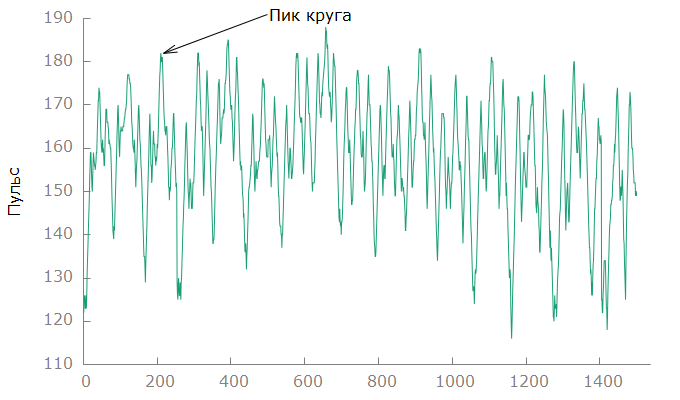
\includegraphics[width=0.5\linewidth]{../[graphics]/hr_graph}
	\caption{График зависимой переменной Пульс}
	\label{fig:hr_graph}
\end{figure}

% Анализ автокорреляции
\textbf{\textit{Анализ автокорреляции}}

\begin{figure}[H]
	\centering
	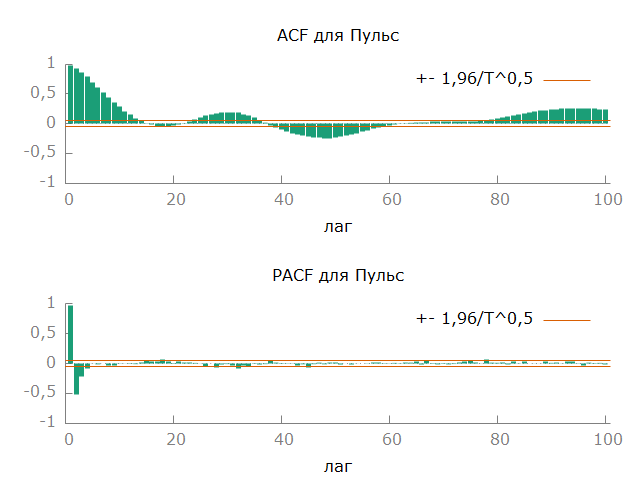
\includegraphics[width=0.5\linewidth]{../[graphics]/hr_acf_100}
	\caption{Графики ACF и PACF зависимой переменной Пульс}
	\label{fig:hr_acf_100}
\end{figure}

График автокорреляции (рис. \ref{fig:hr_acf_100}) убывает медленно, предполагается наличие тренда. На графике видны колебания с периодом в 2 минуты (лаг 30), 3 минуты (лаг 45) и 6 минут (лаг 88). При анализе графика значений зависимой переменной (рис. \ref{fig:hr_graph}) также хорошо видны колебания в 6 минут. По виду графика можно говорить о наличии циклического тренда с периодом, равным среднему времени прохождения спортсменом круга (около 6 минут).

% Анализ спектрограммы
\textbf{\textit{Анализ спектрограммы}}

\begin{figure}[H]
	\centering
	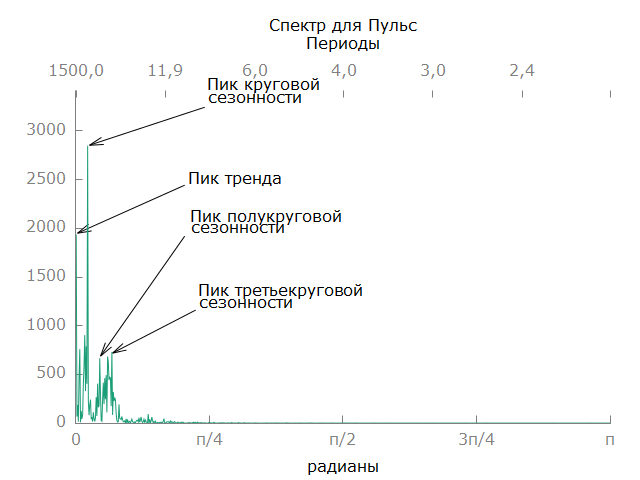
\includegraphics[width=0.5\linewidth]{../[graphics]/hr_spectr}
	\caption{График периодограммы зависимой переменной Пульс}
	\label{fig:hr_spectr}
\end{figure}

При анализе графика (рис. \ref{fig:hr_spectr}) видны пики вблизи нулевой частоты, они свидетельствуют о потенциальном наличии долгосрочного тренда. На графике также видны несколько пиков в циклической области спектра. 
В циклической части спектра на частоте $f = 0,07193 \approx \frac{2 \pi}{87}$ значение спектральной частоты равно $Sd = 2814,4$, указанная частота соответствует периоду 6 минут (среднее время прохождения одного круга).
На частоте $f = 0,20309 \approx \frac{2 \pi}{31}$ значение спектральной частоты равно $Sd = 1167,8$, указанная частота соответствует периоду в 2 минуты (треть круга).
Пиков в сезонной части спектра нет. 
Гармоническая составляющая в указанном ряду является хорошо выраженной.

\textbf{\textit{Анализ стационарности с использованием критерия Dickey-Fuller}}

\begin{table}[H]
	\begin{center}
		\begin{tabular}{|l|l|}
			\hline
			Тип теста &p-value \\
			\hline
			Без константы &0,641 \\
			\hline
			С константой &0 \\
			\hline
			С константой и трендом &0 \\
			\hline
			1 разность, без константы & 0\\
			\hline
			1 разность, с константой & 0\\
			\hline
			1 разность, с констаной и трендом & 0\\
			\hline
		\end{tabular}
	\end{center}
	\caption{Тест Дики-Фуллера для переменной Пульс.}
	\label{tab:DFhr}
\end{table}

По результатам теста (табл. \ref{tab:DFhr}) видно, что исходный ряд с измерениями частоты пульса не является стационарным: нулевая гипотеза о наличии единичного корня не была отвергнута для теста без константы на $5\%$ уровне значимости. После взятия первой разности по результатам всех трёх типов теста Дики-Фуллера нулевая гипотеза о наличии единичного корня была отвергнута в пользу альтернативной: ряд является стационарным, единичных корней нет. Таким образом, временной ряд частоты пульса имеет 1 порядок интегрируемости. 

%Выводы
\textbf{\textit{Выводы}}

Наличие долгосрочного тренда зависимой переменной Пульса объясняется тем, что с течением времени тренировки спортсмен устает, вследствие чего пульс постепенно увеличивается. Наличие циклического тренда в 6 минут объясняется тем, что рельеф местности каждый круг повторяется. Наличие циклической частоты с периодом, равным в 2 минуты (треть круга) связано с периодичной сменой техники передвижения: при увеличении высоты, то есть движении в подъём, спортсмен прикладывает больше усилий и, соответственно, его пульс учащается, при уменьшении высоты спортсмен движется со спуска, для чего затрачивает гораздо меньше усилий, и частота его пульса становится ниже. Ряд не является стационарным, но становится таким после взятия 1 разности.%TODO

\subsection{Независимые переменные}
\subsubsection{Высота}

В качестве первой независимой переменной была рассмотрена высота над уровнем моря (ns1ele).
% Определение
\begin{figure}[H]
	\centering
	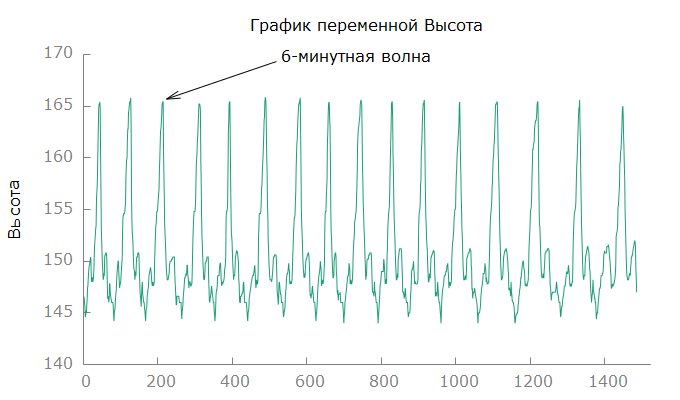
\includegraphics[width=0.5\linewidth]{../[graphics]/ele_graph}
	\caption{График переменной Высота}
	\label{fig:ele_graph}
\end{figure}

% Анализ автокорреляции
\textbf{\textit{Анализ автокорреляции}}

\begin{figure}[H]
	\centering
	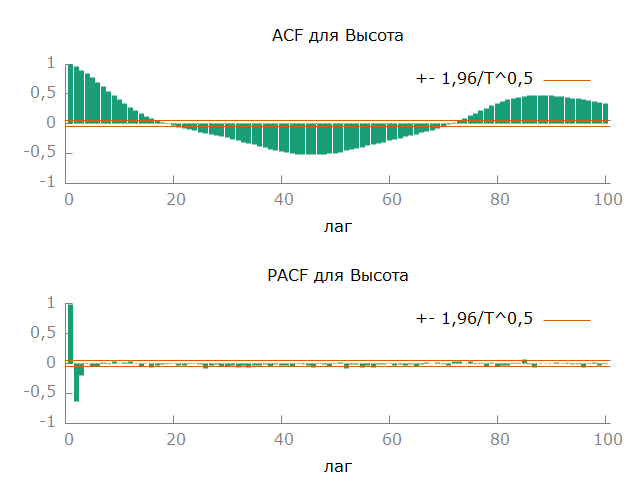
\includegraphics[width=0.5\linewidth]{../[graphics]/ele_acf_100}
	\caption{Графики ACF и PACF переменной Высота}
	\label{fig:ele_acf_100}
\end{figure}

График автокорреляции (рис. \ref{fig:ele_acf_100}) убывает медленно, предполагается наличие тренда. На графике видны колебания с периодом полкруга (3 минуты) и круг (6 минут). При анализе графика значений переменной (рис. \ref{fig:ele_graph}) также хорошо видны колебания с периодом в 6 минут. По виду графика можно говорить о наличии циклического тренда с периодом, равным среднему времени прохождения спортсменом круга.

% Анализ спектрограммы
\textbf{\textit{Анализ спектрограммы}}

\begin{figure}[H]
	\centering
	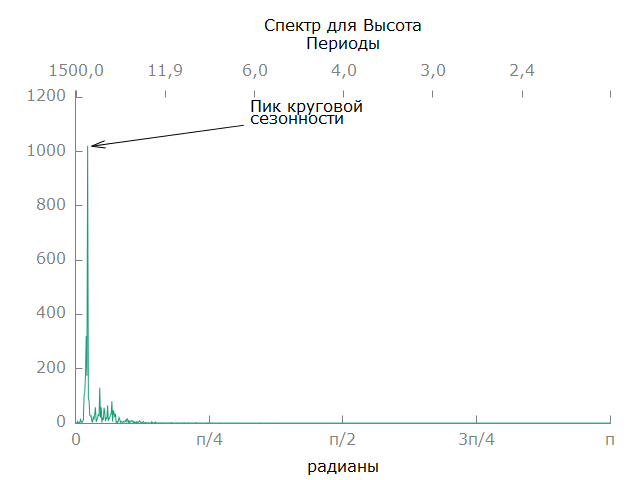
\includegraphics[width=0.5\linewidth]{../[graphics]/ele_spectr}
	\caption{График периодограммы переменной Высота}
	\label{fig:ele_spectr}
\end{figure}

При анализе графика (рис. \ref{fig:hr_spectr}) видно, что пики вблизи нулевой частоты отсутствуют, долгосрочного тренда нет. На графике отсутствуют пики в сезонной области спектра. 
В циклической части спектра на частоте $f = 0,07193 \approx \frac{2 \pi}{87}$ значение спектральной частоты равно $Sd = 938,12$, указанная частота соответствует периоду в 6 минут. 
В циклической части спектра на частоте $f = 0,14386 \approx \frac{2 \pi}{44}$ значение спектральной частоты равно $Sd = 129,12$, указанная частота соответствует периоду в 3 минуты.
В циклической части спектра на частоте $f = 0,22425 \approx \frac{2 \pi}{28}$ значение спектральной частоты равно $Sd = 97,627$, указанная частота соответствует периоду в 2 минуты.
У данного ряда есть ярковыраженная циклическая составляющая.
Также имеются другие неярковыраженные пики в циклической части спектра.

\textbf{\textit{Анализ стационарности с использованием критерия Dickey-Fuller}}

\begin{table}[H]
	\begin{center}
		\begin{tabular}{|l|l|}
			\hline
			Тип теста &p-value \\
			\hline
			Без константы &0,603 \\
			\hline
			С константой &0 \\
			\hline
			С константой и трендом &0 \\
			\hline
			1 разность, без константы & 0\\
			\hline
			1 разность, с константой & 0\\
			\hline
			1 разность, с констаной и трендом & 0\\
			\hline
		\end{tabular}
	\end{center}
	\caption{Тест Дики-Фуллера для переменной Высота.}
	\label{tab:DFele}
\end{table}

По результатам теста (табл. \ref{tab:DFele}) видно, что исходный ряд с измерениями высоты не является стационарным: нулевая гипотеза о наличии единичного корня не была отвергнута для теста без константы на $5\%$ уровне значимости. После взятия первой разности по результатам всех трёх типов теста Дики-Фуллера нулевая гипотеза о наличии единичного корня была отвергнута в пользу альтернативной: ряд является стационарным, единичных корней нет. Таким образом, временной ряд высоты имеет 1 порядок интегрируемости. 

%Выводы
\textbf{\textit{Выводы}}

Долгосрочного тренда в рассматриваемом ряде быть не должно: спортсмен каждый круг проезжал по одной и той же территории, высота не изменялась. Однако заметен циклический тренд с периодом в 6 минут. Наличие циклического тренда объясняется тем, что рельеф местности каждый круг повторяется. Однако в изменениях высоты могут присутствовать незначительные колебания из-за того, что спортсмен каждый раз мог выбирать незначительно отличающуюся траекторию. Ряд не является стационарным, но становится таким после взятия 1 разности.

\subsubsection{Каденс}

В качестве второй независимой переменной была рассмотрена частота шагов (ns2cad).
% Определение
\begin{figure}[H]
	\centering
	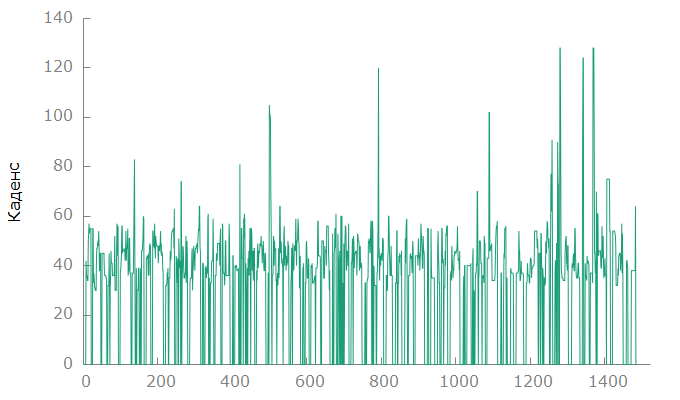
\includegraphics[width=0.5\linewidth]{../[graphics]/cad_graph}
	\caption{График переменной Каденс}
	\label{fig:cad_graph}
\end{figure}

% Анализ автокорреляции
\textbf{\textit{Анализ автокорреляции}}

\begin{figure}[H]
	\centering
	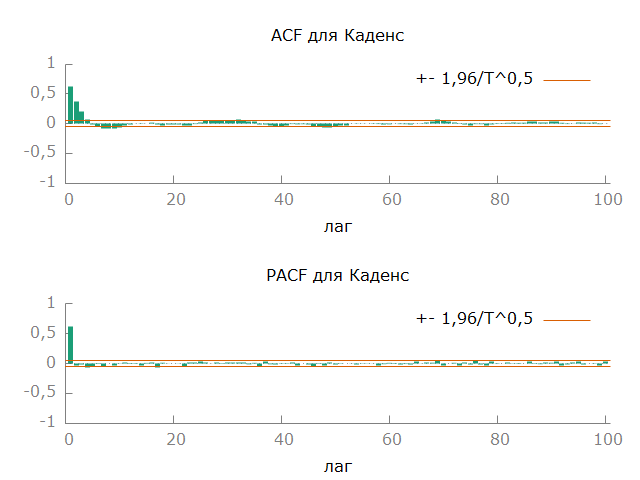
\includegraphics[width=0.5\linewidth]{../[graphics]/cad_acf_100}
	\caption{Графики ACF и PACF переменной Каденс}
	\label{fig:cad_acf_100}
\end{figure}

График автокорреляции (рис. \ref{fig:cad_acf_100}) убывает быстро, предполагается отсутствие тренда. Ярко выраженных периодических затухающих колебаний не выявлено. Указанные замечания также соотносятся с графиком значений переменной (рис. \ref{fig:cad_graph}).

% Анализ спектрограммы
\textbf{\textit{Анализ спектрограммы}}

\begin{figure}[H]
	\centering
	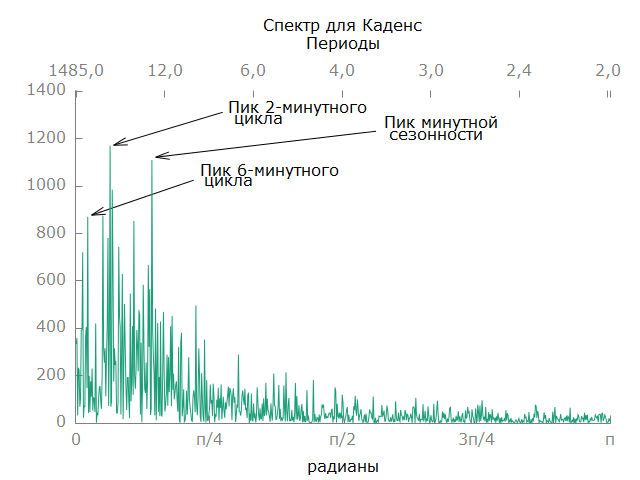
\includegraphics[width=0.5\linewidth]{../[graphics]/cad_spectr}
	\caption{График периодограммы переменной Каденс}
	\label{fig:cad_spectr}
\end{figure}

При анализе графика (рис. \ref{fig:cad_spectr}) видно, что пики вблизи нулевой частоты отсутствуют, долгосрочного тренда нет. На графике присутствуют пики в циклической области спектра. 
В циклической части спектра на частоте $f = 0,07193 \approx \frac{2 \pi}{87}$ значение спектральной частоты равно $Sd = 870,59$, указанная частота соответствует периоду в 6 минут.
В циклической части спектра на частоте $f = 0,20309 \approx \frac{2 \pi}{31}$ значение спектральной частоты равно $Sd = 1170,6$, указанная частота соответствует периоду в 2 минуты.
В сезонной части спектра на частоте $f = 0,44850 \approx \frac{2 \pi}{14}$ значение спектральной частоты равно $Sd = 1110,2$, указанная частота соответствует периоду в 1 минуту.
Также имеются другие пики в циклической и сезонной частях спектра.

\textbf{\textit{Анализ стационарности с использованием критерия Dickey-Fuller}}

\begin{table}[H]
	\begin{center}
		\begin{tabular}{|l|l|}
			\hline
			Тип теста &p-value \\
			\hline
			Без константы &0,076 \\
			\hline
			С константой &0 \\
			\hline
			С константой и трендом &0 \\
			\hline
			1 разность, без константы & 0\\
			\hline
			1 разность, с константой & 0\\
			\hline
			1 разность, с констаной и трендом & 0\\
			\hline
		\end{tabular}
	\end{center}
	\caption{Тест Дики-Фуллера для переменной Каденс.}
	\label{tab:DFcad}
\end{table}

По результатам теста (табл. \ref{tab:DFcad}) видно, что исходный ряд с измерениями каденса не является стационарным: нулевая гипотеза о наличии единичного корня не была отвергнута для теста без константы на $5\%$ уровне значимости. После взятия первой разности по результатам всех трёх типов теста Дики-Фуллера нулевая гипотеза о наличии единичного корня была отвергнута в пользу альтернативной: ряд является стационарным, единичных корней нет. Таким образом, временной ряд каденса имеет 1 порядок интегрируемости. 


%Выводы
\textbf{\textit{Выводы}}

Отсутствие тренда связано с тем, что используемая в конкретный момент техника передвижения спортсмена практически не зависит от техники, используемой в предыдущие моменты времени.
Наличие частот с периодами в 1 и 2 минуты связано с периодичностью применяемой техники передвижения: при движении в подъём прокат на одной ноге (1 шаг) спортсмена становится короче, в связи с этим частота шагов увеличивается по сравнению с движением по ровной местности, при движении со спуска в лыжне спортсмен практически не совершает шагов, поэтому частота шагов иногда становится нулевой. Ряд не является стационарным, но становится таким после взятия 1 разности. %TODO

\subsubsection{Сезонные переменные}
Анализ зависимой переменной не выявил наличие гармонических составляющих с периодами, меньшими минуты.

\section{Выделение трендов}
Начнем с выделения циклических трендов, поскольку они являются наиболее четко выраженными на графиках переменных.

\subsection{Удаление циклического тренда}
Для удаления циклических трендов будем использовать гармонические функции. Из анализа спектрограмм следует, что в рядах присутствуют периодические составляющие с периодами 6 минут, 3 минуты, 2 минуты и 1 минута. Также рассматриваются дополнительные частоты, в которых спектральная частота принимает большие значения. Всего было выявлено 14 частот, в которых замечены высокие значения спектральной частоты (далее нумерация введенных переменных-гармоник соответствует указанному порядку): $$\frac{2 \pi}{297}, \frac{2 \pi}{248}, \frac{2 \pi}{124}, \frac{2 \pi}{114}, \frac{2 \pi}{106}, \frac{2 \pi}{99}, \frac{2 \pi}{93}, \frac{2 \pi}{87}, \frac{2 \pi}{44}, \frac{2 \pi}{36}, \frac{2 \pi}{33}, \frac{2 \pi}{31}, \frac{2 \pi}{28}, \frac{2 \pi}{14}.$$

\subsubsection{Зависимая переменная Пульс}
Построим линейную регрессию переменной Пульс на гармониках для указанных выше частот. Результаты расчетов приведены в таблице ниже. Все частоты за исключением $\frac{2 \pi}{14}$ получились значимыми.

Нами использовалась робастная оценка стандартных ошибок HAC (heteroskedasticity \\ autocorrelated consistent, стандартные ошибки в форме Ньюи-Уеста) - оценка является состоятельной при гетероскедастичности и автокорреляции. Данный метод робастной оценки ковариационной матрицы широко применяется к временным рядам, когда данные для построения модели МНК автокоррелированы. В частности, Gretl по умолчанию использует оценку HAC к временным рядам. Для перекрестных данных в Gretl применяется HCCME (heteroskedasticity-consistent covariance matrix estimator, стандартные ошибки в форме Уайта) - оценка является состоятельной при гетероскедастичности. Для применения HCCME в Gretl существует несколько вариантов: HC0, HC1, HC2, HC3. \footnote{Cottrell A., Lucchetti R. Gretl User’s Guide: GNU Regression, Econometrics and Time-Series Library. 2016 //Software and documentation are available at http://gretl. sourceforge. net. – 2014.}


\begin{table}[H]
\begin{center}
	
	Удаление циклического тренда зависимой переменной: МНК, использованы наблюдения 1--1485\\
	Зависимая переменная: ns2hr\\
	Стандартные ошибки HAC, ширина окна 8 (Ядро Бартлетта (Bartlett))
	
	\vspace{1em}
	
	\begin{tabular}{lr@{,}lr@{,}lr@{,}lr@{,}l}
		&
		\multicolumn{2}{c}{Коэффициент} &
		\multicolumn{2}{c}{Ст.\ ошибка} &
		\multicolumn{2}{c}{$t$-статистика} &
		\multicolumn{2}{c}{P-значение} \\[1ex]
		const &		157&743 &		0&656379 &		240&3 &		0&0000 \\
		c1 &		0&00308109 &		0&775609 &		0&003972 &		0&9968 \\
		s1 &		2&96469 &		1&06039 &		2&796 &		0&0052 \\
		c2 &		$-$3&45727 &		0&887961 &		$-$3&893 &		0&0001 \\
		s2 &		$-$0&451657 &		0&973332 &		$-$0&4640 &		0&6427 \\
		c3 &		2&15391 &		0&921646 &		2&337 &		0&0196 \\
		s3 &		$-$2&14060 &		0&900929 &		$-$2&376 &		0&0176 \\
		c4 &		0&0245971 &		0&900507 &		0&02731 &		0&9782 \\
		s4 &		$-$3&77913 &		0&940082 &		$-$4&020 &		0&0001 \\
		c5 &		$-$1&86244 &		0&969532 &		$-$1&921 &		0&0549 \\
		s5 &		$-$1&60608 &		0&885599 &		$-$1&814 &		0&0700 \\
		c6 &		0&445651 &		0&903548 &		0&4932 &		0&6219 \\
		s6 &		3&29686 &		0&951217 &		3&466 &		0&0005 \\
		c7 &		1&21006 &		0&841936 &		1&437 &		0&1509 \\
		s7 &		3&48608 &		0&985024 &		3&539 &		0&0004 \\
		c8 &		$-$6&15996 &		0&870829 &		$-$7&074 &		0&0000 \\
		s8 &		$-$3&03899 &		0&929493 &		$-$3&270 &		0&0011 \\
		c9 &		$-$1&63113 &		0&899804 &		$-$1&813 &		0&0701 \\
		s9 &		$-$2&23476 &		0&881073 &		$-$2&536 &		0&0113 \\
		c10 &		1&71114 &		0&806446 &		2&122 &		0&0340 \\
		s10 &		$-$3&52976 &		0&901322 &		$-$3&916 &		0&0001 \\
		c11 &		$-$3&48449 &		0&887674 &		$-$3&925 &		0&0001 \\
		s11 &		$-$2&09333 &		0&830548 &		$-$2&520 &		0&0118 \\
		c12 &		1&54375 &		0&853418 &		1&809 &		0&0707 \\
		s12 &		$-$4&16356 &		0&822035 &		$-$5&065 &		0&0000 \\
		c13 &		$-$2&13518 &		0&839731 &		$-$2&543 &		0&0111 \\
		s13 &		$-$2&01712 &		0&806885 &		$-$2&500 &		0&0125 \\
		c14 &		0&900906 &		0&576660 &		1&562 &		0&1184 \\
		s14 &		0&213285 &		0&571939 &		0&3729 &		0&7093 \\
	\end{tabular}
	
	\vspace{1ex}
	\begin{tabular}{lrlr}
		Среднее зав. перемен &  157,6983 & Ст. откл. зав. перемен &  13,68422 \\
		Сумма кв. остатков &  137168,6 & Ст. ошибка модели &  9,706143 \\
		$R^2$ &  0,506394 & Исправленный $R^2$ &  0,496901 \\
		$F(28, 1456)$ &  17,73434 & Р-значение($F$) &  9,59\textrm{e--74} \\
		Лог. правдоподобие & $-$5467,527 & Крит. Акаике &  10993,05 \\
		Крит. Шварца &  11146,85 & Hannan--Quinn &  11050,38 \\
		$\hat{\rho}$ &  0,963471 & Durbin--Watson &  0,072530 \\
	\end{tabular}
\end{center}
\caption{Удаление циклического тренда зависимой переменной Пульс с корректировкой на автокорреляцию.}
\label{tab:table1}
\end{table}

Графики расчетных значений модели и остаточной разности представлены соответственно на рис.\ref{fig:hr_trend0} и рис.\ref{fig:hr_error0}. По графику остаточной разности можно сказать, что точек перемены знака много. Значит сильной статистической связи между соседними значениями временного ряда нет. 

\begin{figure}[H]
	\centering
\begin{minipage}{.5\textwidth}
	\centering
	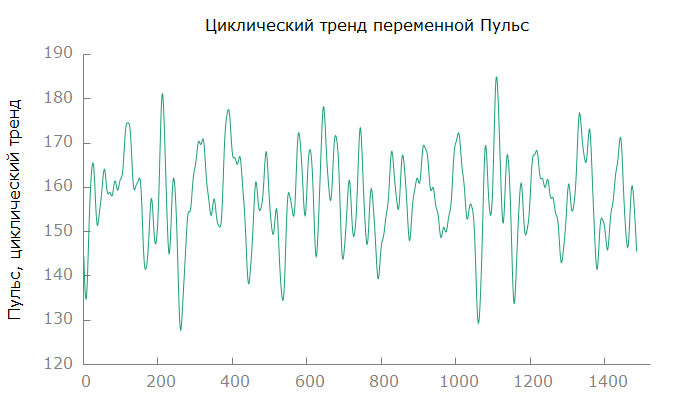
\includegraphics[width=\linewidth]{../[graphics]/hr_trend0.png}
	\caption{Циклический тренд переменной Пульс}
	\label{fig:hr_trend0}
\end{minipage}%
\begin{minipage}{.5\textwidth}
	\centering
	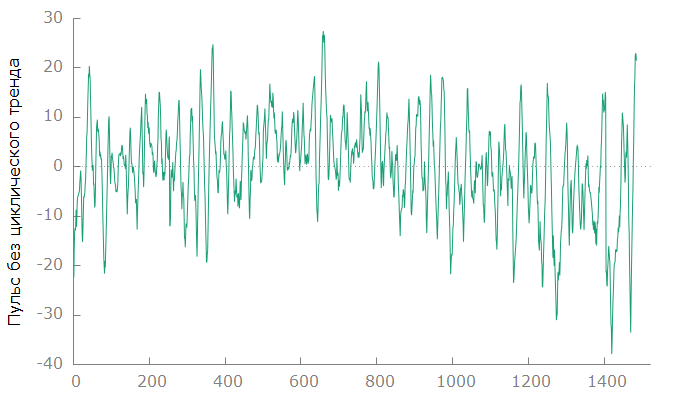
\includegraphics[width=\linewidth]{../[graphics]/hr_error0.png}
	\caption{Пульс без циклического тренда}
	\label{fig:hr_error0}
\end{minipage}
\end{figure}

По графику спектра переменной Пульс без циклического тренда (рис.\ref{fig:hr_error0_spectr}) видно, что мы действительно избавились от циклической составляющей.

\begin{figure}[H]
	\centering
	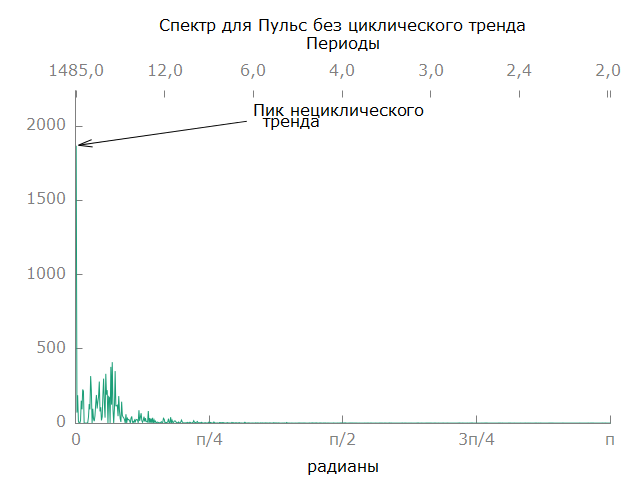
\includegraphics[width=0.5\linewidth]{../[graphics]/hr_error0_spectr.png}
	\caption{График спектра переменной Пульс без циклического тренда}
	\label{fig:hr_error0_spectr}
\end{figure}

Для дальнейшего анализа будем использовать остаточную разность hr\_error0, полученную из переменной Пульс после удаления циклического тренда.

\subsubsection{Независимые переменные}
Аналогично предыдущему пункту построим линейные регрессии для независимых переменных Высота и Каденс на указанных ранее гармониках. 
Для переменной Высота все частоты кроме $\frac{2 \pi}{248}, \frac{2 \pi}{14}$ получились значимыми. Для переменной Каденс значимыми оказались частоты $\frac{2 \pi}{106}, \frac{2 \pi}{99}, \frac{2 \pi}{87}, \frac{2 \pi}{44}, \frac{2 \pi}{33}, \frac{2 \pi}{31}, \frac{2 \pi}{14}$.

По графику спектра переменной Высота без циклического тренда (рис.\ref{fig:ele_error0_spectr}) видно, что пиков стало меньше, но окончательно избавиться от циклической составляющей не удалось.

\begin{figure}[H]
	\centering
	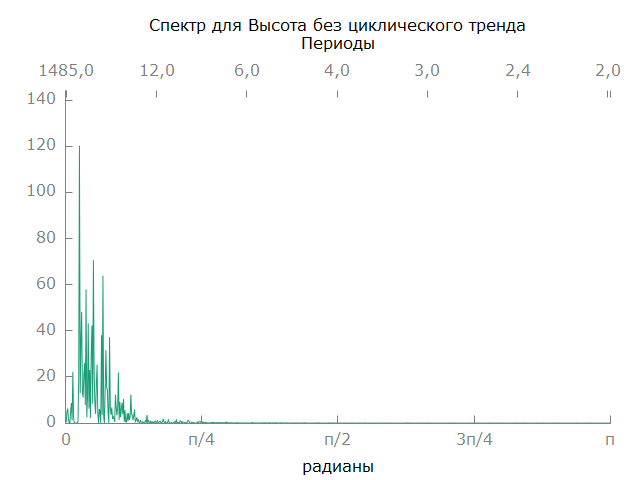
\includegraphics[width=0.5\linewidth]{../[graphics]/ele_error0_spectr.png}
	\caption{График спектра переменной Высота без циклического тренда}
	\label{fig:ele_error0_spectr}
\end{figure}

По графику спектра переменной Каденс без циклического тренда (рис.\ref{fig:cad_error0_spectr}) видно, что пиков стало меньше, но окончательно избавиться от циклической составляющей не удалось.

\begin{figure}[H]
	\centering
	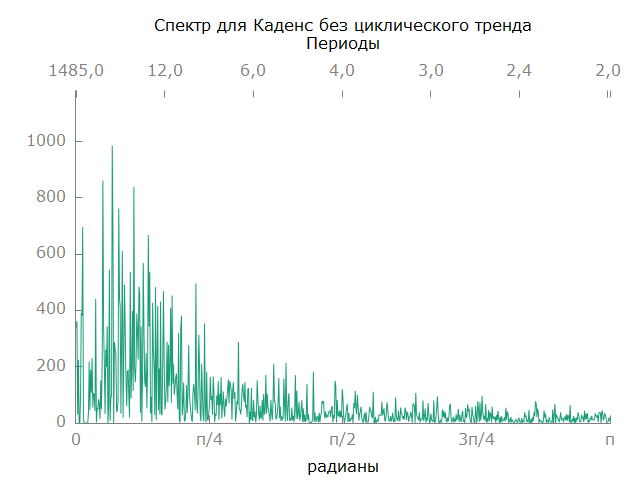
\includegraphics[width=0.5\linewidth]{../[graphics]/cad_error0_spectr.png}
	\caption{График спектра переменной Каденс без циклического тренда}
	\label{fig:cad_error0_spectr}
\end{figure}

Для дальнейшего анализа будем использовать остаточные разности ele\_error0 и cad\_error0, полученные соответственно из переменных Высота и Каденс после удаления циклического тренда.

\subsection{Выделение полиномиальных трендов}
Спектральный анализ показал наличие нециклического тренда для переменной Пульс. Избавимся от такого тренда с помощью полиномиальной модели. Степень полинома будем выбирать с помощью постепенного наращивания степени, пока коэффициент при старшей степени не станет незначимым. Удаление начнем с зависимой переменной hr\_error0 (перемененная Пульс без циклического тренда).

\subsubsection{Зависимая переменная Пульс}

Указанным выше способом удалось выделить тренд 2 степени. Результаты расчетов приведены в таблице ниже. При построении модели использовались корректировки Ньюи-Уеста HAC.

\begin{table}[H]
	\begin{center}
		
		Удаление полиномиального тренда переменной hr\_error0:
		МНК, использованы наблюдения 1--1485\\
		Зависимая переменная: hr\_error0\\
		Стандартные ошибки HAC, ширина окна 8 (Ядро Бартлетта (Bartlett))
		
		\vspace{1em}
		
		\begin{tabular}{lr@{,}lr@{,}lr@{,}lr@{,}l}
			&
			\multicolumn{2}{c}{Коэффициент} &
			\multicolumn{2}{c}{Ст.\ ошибка} &
			\multicolumn{2}{c}{$t$-статистика} &
			\multicolumn{2}{c}{P-значение} \\[1ex]
			const &			$-$2&41303 &			1&70193 &			$-$1&418 &			0&1565 \\
			t &			0&0211497 &			0&00578487 &			3&656 &			0&0003 \\
			t2 &			$-$1&80768\textrm{e--005} &			4&13261\textrm{e--006} &			$-$4&374 &			0&0000 \\
		\end{tabular}
		
		\vspace{1ex}
		\begin{tabular}{lrlr}
			Среднее зав. перемен &  8,53\textrm{e--14} & Ст. откл. зав. перемен &  9,614140 \\
			Сумма кв. остатков &  115153,7 & Ст. ошибка модели &  8,814847 \\
			$R^2$ &  0,160496 & Исправленный $R^2$ &  0,159363 \\
			$F(2, 1482)$ &  12,17696 & Р-значение($F$) &  5,68\textrm{e--06} \\
			Лог. правдоподобие & $-$5337,632 & Крит. Акаике &  10681,26 \\
			Крит. Шварца &  10697,17 & Hannan--Quinn &  10687,19 \\
			$\hat{\rho}$ &  0,959238 & Durbin--Watson &  0,086404 \\
		\end{tabular}
	\end{center}
\caption{Удаление полиномиального тренда зависимой переменной Пульс с корректировкой на автокорреляцию.}
\label{tab:table2}
\end{table}

При анализе спектрограммы на графике \ref{fig:hr_error1_spectr} видно, что с помощью удаления полиномиального тренда 2 степени удалось избавиться от нециклического тренда.

\begin{figure}[H]
	\centering
	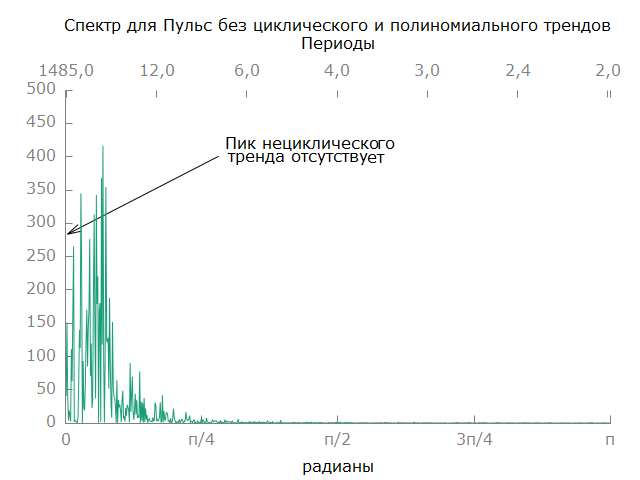
\includegraphics[width=0.5\linewidth]{../[graphics]/hr_error1_spectr.png}
	\caption{График спектра переменной Пульс без циклического и полиномиального трендов}
	\label{fig:hr_error1_spectr}
\end{figure}

По графику переменной Пульс без циклического и полиномиального трендов (рис. \ref{fig:hr_error1}) можно сказать, что долгосрочного тренда в данном ряду не заметно, однако видно циклические составляющие. По графику \ref{fig:hr_error1} можно сказать, что точек перемены знака много. Значит сильной статистической связи между соседними значениями временного ряда нет. Это подтверждается графиком автокорреляции ниже.

\begin{figure}[H]
	\centering
	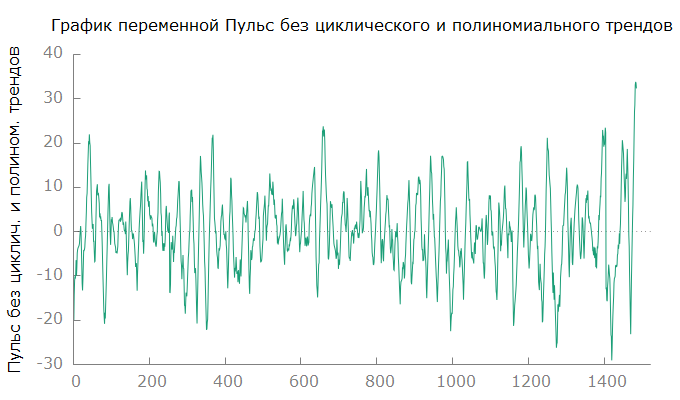
\includegraphics[width=0.5\linewidth]{../[graphics]/hr_error1.png}
	\caption{График переменной Пульс без циклического и полиномиального трендов}
	\label{fig:hr_error1}
\end{figure}

График автокорреляции (рис. \ref{fig:hr_error1_acf_100}) убывает быстро, полиномиальный тренд отсутствует.

\begin{figure}[H]
	\centering
	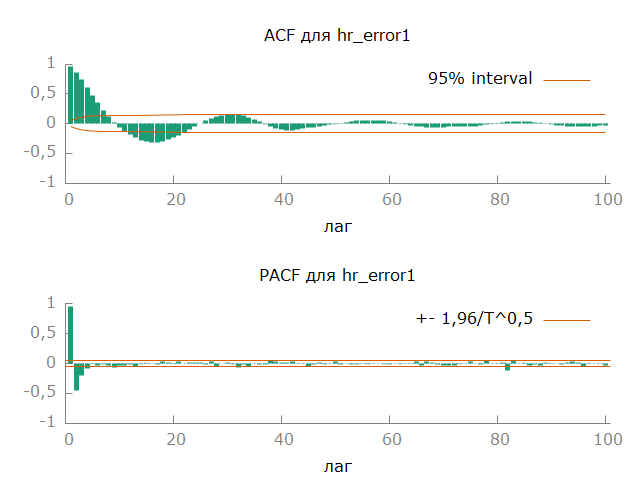
\includegraphics[width=0.5\linewidth]{../[graphics]/hr_error1_acf_100.png}
	\caption{Графики ACF и PACF переменной Пульс без циклического и полиномиального трендов}
	\label{fig:hr_error1_acf_100}
\end{figure}

Далее в работе будем использовать остаточную разность hr\_error1 после удаления полиномиального тренда из переменной hr\_error0.

\subsubsection{Независимые переменные}

С помощью аналогичной процедуры удалим нециклический тренд из переменных ele\_error0 (переменная Высота без циклического тренда) и cad\_error0 (переменная Каденс без циклического тренда). Как и ожидалось, коэффициенты перед степенями полинома оказались незначимыми, поскольку в переменных Высота и Каденс отсутствует нециклический тренд.

При анализе спектрограмм на графиках \ref{fig:ele_error1_spectr} и \ref{fig:cad_error1_spectr} видно, что спектры для переменных Высота и Каденс практически не изменились ввиду отсутствия в этих переменных полиномиальных трендов.

\begin{figure}[H]
	\centering
	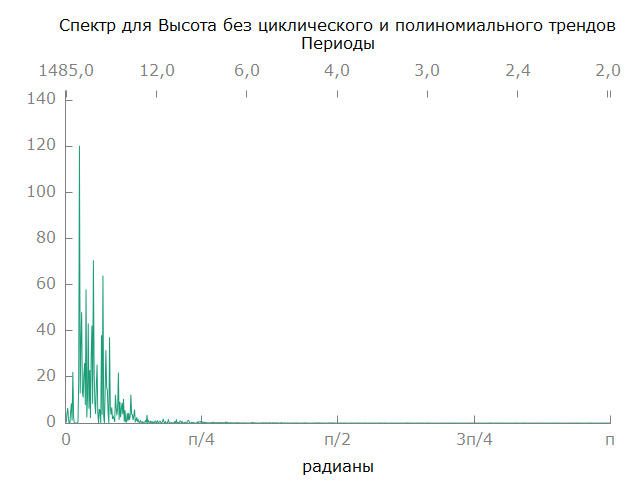
\includegraphics[width=0.5\linewidth]{../[graphics]/ele_error1_spectr.png}
	\caption{График спектра переменной Высота без циклического и полиномиального трендов}
	\label{fig:ele_error1_spectr}
\end{figure}

\begin{figure}[H]
	\centering
	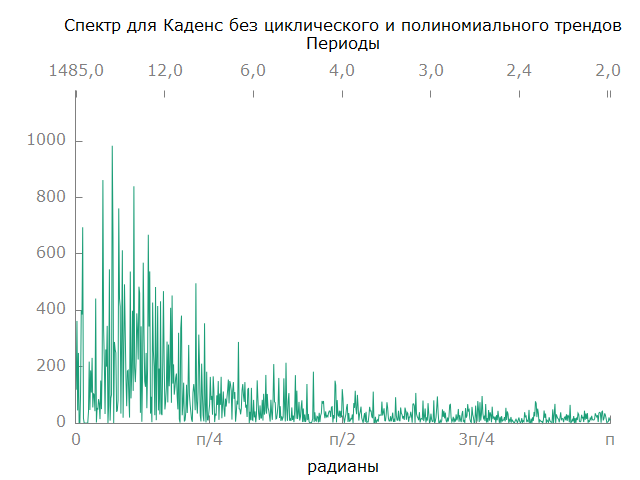
\includegraphics[width=0.5\linewidth]{../[graphics]/cad_error1_spectr.png}
	\caption{График спектра переменной Каденс без циклического и полиномиального трендов}
	\label{fig:cad_error1_spectr}
\end{figure}

По графикам переменных Высота и Каденс без циклического и полиномиального трендов (рис. \ref{fig:ele_error1}, рис. \ref{fig:cad_error1}) можно сказать, что долгосрочного тренда в указанных рядах не обнаружено, однако заметно циклические составляющие. По графикам \ref{fig:ele_error1} и \ref{fig:cad_error1} также можно сказать, что точек перемены знака много. Значит сильной статистической связи между соседними значениями временных рядов нет. Это подтверждается графиками автокорреляции ниже.

\begin{figure}[H]
	\centering
	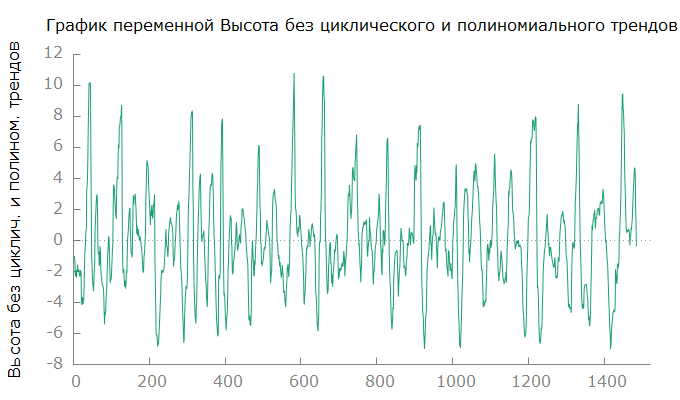
\includegraphics[width=0.5\linewidth]{../[graphics]/ele_error1.png}
	\caption{График переменной Высота без циклического и полиномиального трендов}
	\label{fig:ele_error1}
\end{figure}

\begin{figure}[H]
	\centering
	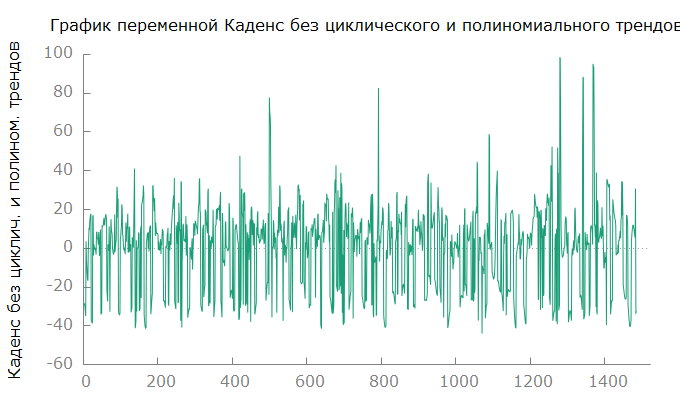
\includegraphics[width=0.5\linewidth]{../[graphics]/cad_error1.png}
	\caption{График переменной Каденс без циклического и полиномиального трендов}
	\label{fig:cad_error1}
\end{figure}

Графики автокорреляции (рис. \ref{fig:ele_error1_acf_100}, рис. \ref{fig:cad_error1_acf_100}) убывают быстро, полиномиальный тренд отсутствует.

\begin{figure}[H]
	\centering
	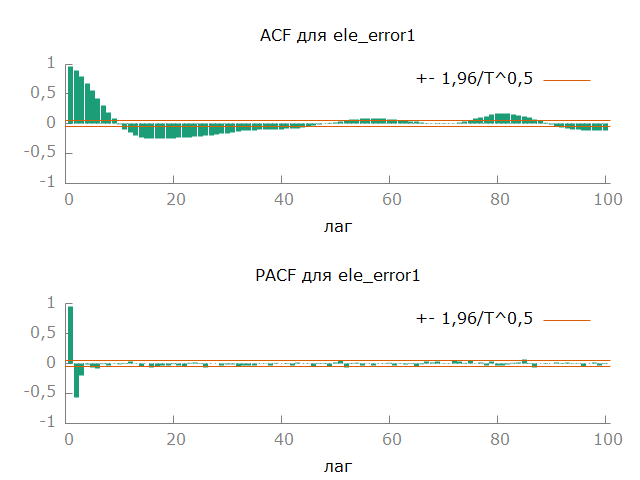
\includegraphics[width=0.5\linewidth]{../[graphics]/ele_error1_acf_100.png}
	\caption{Графики ACF и PACF переменной Высота без циклического и полиномиального трендов}
	\label{fig:ele_error1_acf_100}
\end{figure}

\begin{figure}[H]
	\centering
	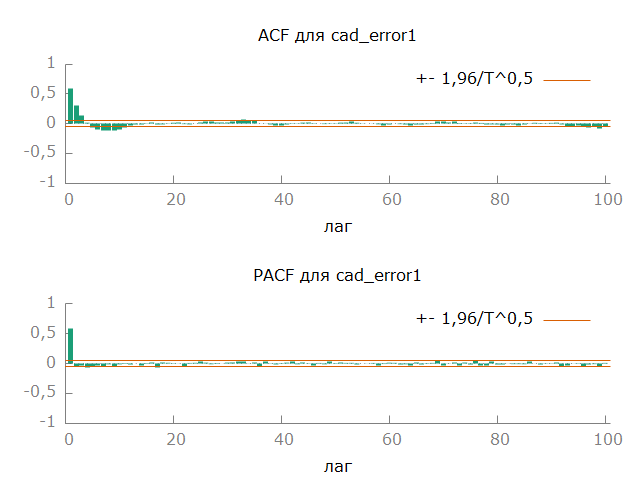
\includegraphics[width=0.5\linewidth]{../[graphics]/cad_error1_acf_100.png}
	\caption{Графики ACF и PACF переменной Каденс без циклического и полиномиального трендов}
	\label{fig:cad_error1_acf_100}
\end{figure}

Далее в работе будем использовать остаточные разности ele\_error1 и cad\_error1 после удаления полиномиального тренда из переменных ele\_error0 и cad\_error0 соответственно.

\section{Автономные динамические модели временных рядов}

\textbf{\textit{Зависимая переменная Пульс}}
		
Построим автономную динамическую модель зависимой переменной. В соответствии с методологией Бокса и Дженкинса проанализируем вид функции автокорреляции и частной автокорреляции для данного ряда после удаления циклического и нециклического трендов. По графику временного ряда (рис. \ref{fig:hr_error1}) видно, что сезонные колебания и тренды отсутствуют. По графикам ACF и PACF переменной Пульс после удаления трендов (рис. \ref{fig:hr_error1_acf_100}) видны пики на первых 2 лагах PACF, а также ненулевые значения на 3 и 4 лагах, по ACF ненулевыми были первые 8 лагов, в связи с этим были проверены модели AR(1), AR(2), AR(3), ARIMA(3,0,1),ARIMA(3,0,2), ARIMA(3,0,3), ARIMA(3,0,4), ARIMA(3,0,5), ARIMA(3,0,6), ARIMA(3,0,7), ARIMA(3,0,8). Также для исходного ряда ns2hr была проверена модель ARIMA(3,1,0), так как ряд порядка интегрируемости 1. Наилучшей моделью по некоррелированности остатков и минимальным значениям критерия Акаике оказалась модель ARIMA(3,0,8), результаты её построения представлены в табл. \ref{tab:ARIMAhr}.

\begin{table}[H]
	\begin{center}
		
		Модель: ARMA, использованы наблюдения 1--1485\\
		Зависимая переменная: hr\_error1\\
		Стандартные ошибки рассчитаны на основе Гессиана
		
		\vspace{1em}
		
		\begin{tabular}{lr@{,}lr@{,}lr@{,}lr@{,}l}
			&
			\multicolumn{2}{c}{Коэффициент} &
			\multicolumn{2}{c}{Ст.\ ошибка} &
			\multicolumn{2}{c}{$z$} &
			\multicolumn{2}{c}{P-значение} \\[1ex]
			const &
			$-$0&0218654 &
			0&602770 &
			$-$0&03627 &
			0&9711 \\
			$\phi_{1}$ &
			2&54408 &
			0&0893881 &
			28&46 &
			0&0000 \\
			$\phi_{2}$ &
			$-$2&17183 &
			0&169052 &
			$-$12&85 &
			0&0000 \\
			$\phi_{3}$ &
			0&609700 &
			0&0835496 &
			7&297 &
			0&0000 \\
			$\theta_{1}$ &
			$-$1&21174 &
			0&0919533 &
			$-$13&18 &
			0&0000 \\
			$\theta_{2}$ &
			0&298957 &
			0&0657692 &
			4&546 &
			0&0000 \\
			$\theta_{3}$ &
			$-$0&00250239 &
			0&0423987 &
			$-$0&05902 &
			0&9529 \\
			$\theta_{4}$ &
			$-$0&0350638 &
			0&0418859 &
			$-$0&8371 &
			0&4025 \\
			$\theta_{5}$ &
			0&0615158 &
			0&0419064 &
			1&468 &
			0&1421 \\
			$\theta_{6}$ &
			0&00945589 &
			0&0412222 &
			0&2294 &
			0&8186 \\
			$\theta_{7}$ &
			$-$0&000653030 &
			0&0404035 &
			$-$0&01616 &
			0&9871 \\
			$\theta_{8}$ &
			0&0862443 &
			0&0330841 &
			2&607 &
			0&0091 \\
		\end{tabular}
		
		\vspace{1ex}
		\begin{tabular}{lrlr}
			Среднее зав. перемен & $-$3,45\textrm{e--16} & Ст. откл. зав. перемен &  8,808905 \\
			Среднее инноваций &  0,006473 & Ст. откл. инноваций &  2,137220 \\
			$R^2$ &  0,941097 & Исправленный $R^2$ &  0,940698 \\
			Лог. правдоподобие & $-$3236,786 & Крит. Акаике &  6499,571 \\
			Крит. Шварца &  6568,512 & Hannan--Quinn &  6525,267 \\
		\end{tabular}
		
		
		\vspace{1em}
		
		\begin{tabular}{llrrrrr}
			& & & Действительная часть & Мнимая часть & Модуль & Частота \\ \hline
			AR \\ 
			& Корень & 1 & $1,5686$ & $0,0000$ & $1,5686$ & $0,0000$ \\ 
			& Корень & 2 & $0,9968$ & $-0,2282$ & $1,0225$ & $-0,0358$ \\ 
			& Корень & 3 & $0,9968$ & $0,2282$ & $1,0225$ & $0,0358$ \\ 
			MA \\ 
			& Корень & 1 & $1,0142$ & $-0,2644$ & $1,0481$ & $-0,0406$ \\ 
			& Корень & 2 & $1,0142$ & $0,2644$ & $1,0481$ & $0,0406$ \\ 
			& Корень & 3 & $-1,4542$ & $-0,6438$ & $1,5903$ & $-0,4337$ \\ 
			& Корень & 4 & $-1,4542$ & $0,6438$ & $1,5903$ & $0,4337$ \\ 
			& Корень & 5 & $0,7539$ & $-1,1509$ & $1,3758$ & $-0,1577$ \\ 
			& Корень & 6 & $0,7539$ & $1,1509$ & $1,3758$ & $0,1577$ \\ 
			& Корень & 7 & $-0,3102$ & $-1,4521$ & $1,4848$ & $-0,2835$ \\ 
			& Корень & 8 & $-0,3102$ & $1,4521$ & $1,4848$ & $0,2835$ \\ \hline
		\end{tabular}
		
	\end{center}
	\caption{Автономная динамическая модель ARIMA(3,0,8) для переменной пульс.}
	\label{tab:ARIMAhr}
\end{table}

Построенная модель описывает 94\% вариации переменной Пульс, не имеет единичных корней, а значит является стационарной и обратимой. Остатки некоррелированны (рис. \ref{fig:hr_arima}).

\begin{figure}[H]
	\centering
	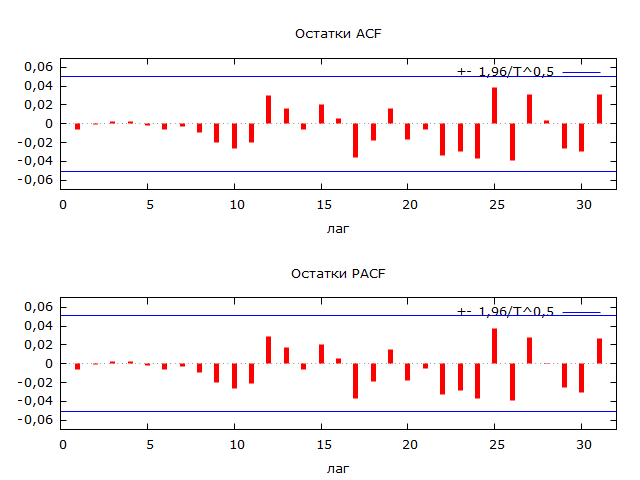
\includegraphics[width=0.5\linewidth]{../[graphics]/hr_arima.png}
	\caption{Графики ACF и PACF остаточной разности модели ARIMA(3,0,8) для переменной Пульс.}
	\label{fig:hr_arima}
\end{figure}

Коэффициенты при $\theta_2-\theta_7$ оказались незначимы, однако модель только с 1 и 8 лагами МА хуже по критерию Акаике и коррелированности остатков. Остановимся на данном варианте модели. Итоговое уравнение имеет вид:
\begin{align*}
&hr\_error1_t =  \underset{(0,09)}{2,54}hr\_error1_{t-1}-\underset{(0,17)}{2,17}hr\_error1_{t-2}+\underset{(0,08)}{0,61}hr\_error1_{t-3}+v_t - \\ &-\underset{(0,09)}{1,21}v_{t-1}+\underset{(0,07)}{0,29}v_{t-2}-\underset{(0,04)}{0,0025}v_{t-3} -\underset{(0,04)}{0,035}v_{t-4}+\underset{(0,04)}{0,06}v_{t-5}+\underset{(0,04)}{0,01}v_{t-6}-\underset{(0,04)}{0,0007}v_{t-7}+\underset{(0,03)}{0,09}v_{t-8}.
\end{align*}

$D[v_t]\approx2,14^2=4,58$.

Оценки коэффициентов приведены с округлением, в скобках указаны стандартные ошибки оценок. В операторной форме данная модель имеет вид:
\begin{align*}
&hr\_error1_t = \\ & = \frac{1-2,54z-2,17z^2+0,61z^3}{1-1,21z+0,29z^2-0,0025z^3-0,035z^4+0,06z^5+0,01z^6-0,0007z^7+0,09z^8}=H(z)v_t.
\end{align*}
где $z$ - оператор запаздывания, $H(z)$ - передаточная функция. Прогноз на 1 шаг вперёд $\hat{u}_{t,1}$ определяется по формуле:
\begin{align*}
&\hat{u}_{t,1}=(H(z)-1)H^{-1}(z)hr\_error1_t= \\
& = \frac{-1,33 z - 2,46 z^2 + 0,6125 z^3 + 0,035 z^4 - 0,06 z^5 - 0,01 z^6 + 0,0007 z^7 - 0,09 z^8}{1-2,54z-2,17z^2+0,61z^3}.
\end{align*}
Или в разностном виде:
\begin{align*}
&\hat{u}_{t,1}-2,54\hat{u}_{t-1,1}-2,17\hat{u}_{t-2,1}+0,61\hat{u}_{t-3,1} = \\
& = -1,33hr\_error1_{t-1} - 2,46 hr\_error1_{t-2} + 0,6125hr\_error1_{t-3} + 0,035hr\_error1_{t-4} - \\
& - 0,06hr\_error1_{t-5} - 0,01 hr\_error1_{t-6} + 0,0007hr\_error1_{t-7} - 0,09hr\_error1_{t-8}.
\end{align*}
Таким образом, доверительный интервал прогноза на один шаг с уровнем доверия 95\% имеет вид: $\left[\hat{u}_{t,t-1}\pm1,96\cdot2,14\right]=\left[\hat{u}_{t,t-1}\pm4,19\right],$ а дисперсия ошибки $D[hr\_error1_t-\hat{u}_{t,t-1}]\approx4,58$.

\section{Оценивание параметров линейной регрессии при наличии автокорреляции у случайной составляющей}

\subsection{Вид модели и гипотезы}
Далее исследуем гипотезы о направлении влияния показателей, очищенных от систематических компонент. Для построения основной модели используем обобщенную модель линейной регрессии (в качестве переменных берем остаточные разности после удаления трендов):
\[hr\_error1 = a_0 + a_1 ele\_error1 + a_2 cad\_error1 + v_t,\]

где $v_t$ - случайная составляющая.

Гипотезу 1 о том, что увеличение высоты статистически связано с увеличением частоты пульса спортсмена, проверим следующим образом. Если гипотеза $H_0$ о том, что увеличение высоты не влияет на частоту пульса, верна, то коэффициент при переменной $ele\_error1$ $a_1 = 0$. Если верна альтернативная гипотеза $H_1$ о том, что увеличение высоты влияет на пульс спортсмена в сторону его увеличения, то $a_1 > 0$.

Гипотезу 2 о том, что увеличение частоты шагов статистически связано с увеличением частоты пульса спортсмена, проверим следующим образом. Если гипотеза $H_0$ о том, что увеличение каденса не влияет на частоту пульса, верна, то коэффициент при переменной $cad\_error1$ $a_2 = 0$. Если верна альтернативная гипотеза $H_1$ о том, что увеличение каденса влияет на пульс спортсмена в сторону его увеличения, то $a_2 > 0$.

\subsection{Построение линейной регрессионной модели методом наименьших квадратов}

\begin{table}[H]
\begin{center}
	
	Основная модель: МНК, использованы наблюдения 1--1485\\
	Зависимая переменная: hr\_error1\\
	Стандартные ошибки HAC, ширина окна 8 (Ядро Бартлетта (Bartlett))
	
	\vspace{1em}
	
	\begin{tabular}{lr@{,}lr@{,}lr@{,}lr@{,}l}
		&
		\multicolumn{2}{c}{Коэффициент} &
		\multicolumn{2}{c}{Ст.\ ошибка} &
		\multicolumn{2}{c}{$t$-статистика} &
		\multicolumn{2}{c}{P-значение} \\[1ex]
		const &
		0&000000 &
		0&514243 &
		0&0000 &
		1&0000 \\
		ele\_error1 &
		1&24162 &
		0&153968 &
		8&064 &
		0&0000 \\
		cad\_error1 &
		$-$0&0156583 &
		0&0152096 &
		$-$1&030 &
		0&3034 \\
	\end{tabular}
	
	\vspace{1ex}
	\begin{tabular}{lrlr}
		Среднее зав. перемен &  0,000000 & Ст. откл. зав. перемен &  8,808905 \\
		Сумма кв. остатков &  92163,11 & Ст. ошибка модели &  7,885958 \\
		$R^2$ &  0,199651 & Исправленный $R^2$ &  0,198571 \\
		$F(2, 1482)$ &  33,49773 & Р-значение($F$) &  5,91\textrm{e--15} \\
		Лог. правдоподобие & $-$5172,272 & Крит. Акаике &  10350,54 \\
		Крит. Шварца &  10366,45 & Hannan--Quinn &  10356,47 \\
		$\hat{\rho}$ &  0,951092 & Durbin--Watson &  0,104092 \\
	\end{tabular}
\end{center}
\caption{Основная модель статистической взаимосвязи между зависимой и независимыми переменными.}
\label{tab:table3}
\end{table}

Построенная линейная регрессионная модель представлена в таблице \ref{tab:table3} (с использованием корректировок Ньюи-Уеста). Только переменная ele\_error1 оказалась значимой, соответствующий коэффициент $a_1 = 1,24 > 0$ положительный. Гипотеза 1 подтверждается. Так, при увеличении высоты на один метр частота пульса увеличится в среднем на 1,24 ударов в минуту для постоянных значений прочих регрессоров.

Однако для переменной cad\_error1 соответствующий коэффициент $a_2 = -0,016 < 0$ отрицателен, но близок к нулю и незначимый. Гипотеза 2 не подтверждается.

Статистика Дарбина-Ватсона значительно меньше 2 и близка к 0. Следовательно, в случайной составляющей $v_t$ есть положительная автокорреляция первого порядка.

\subsection{Уточнение вида модели с учетом наличия автокорреляции в случайной составляющей}
Исследуем остаточную разность основной модели hr\_error2. При анализе графика \ref{fig:hr_error2_acf_100} можно говорить о наличии автокорреляции случайной составляющей $v_t$. Предположительно, будем использовать авторегрессию до 9 порядка (смотрим по значимости коэффициентов частной автокорреляции для разных лагов - оценка автокорреляции значимая до лага 9). Для скользящего среднего порядок может быть около 7 - наблюдается сильная значимость коэффициентов до 7 лага. По графику периодограммы \ref{fig:hr_error2_spectr} можно сказать, что ярко выраженных пиков в сезонной части спектра не выявлено (значимые пики находятся в циклической части спектра) - наша модель не будет учитывать сезонность. 

\begin{figure}[H]
	\centering
	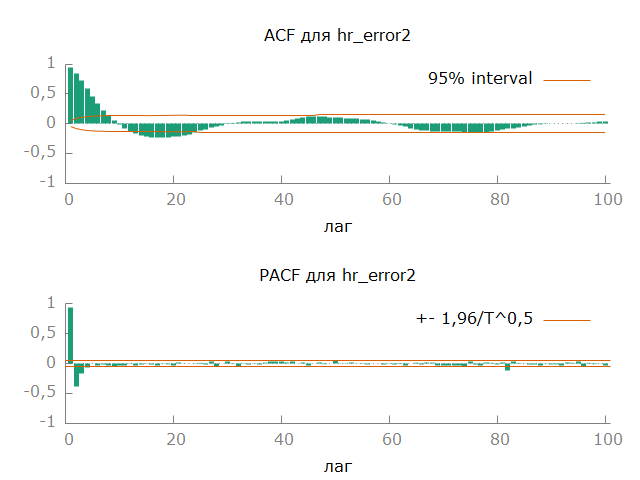
\includegraphics[width=0.5\linewidth]{../[graphics]/hr_error2_acf_100.png}
	\caption{Графики ACF и PACF остаточной разности основной модели}
	\label{fig:hr_error2_acf_100}
\end{figure}

\begin{figure}[H]
	\centering
	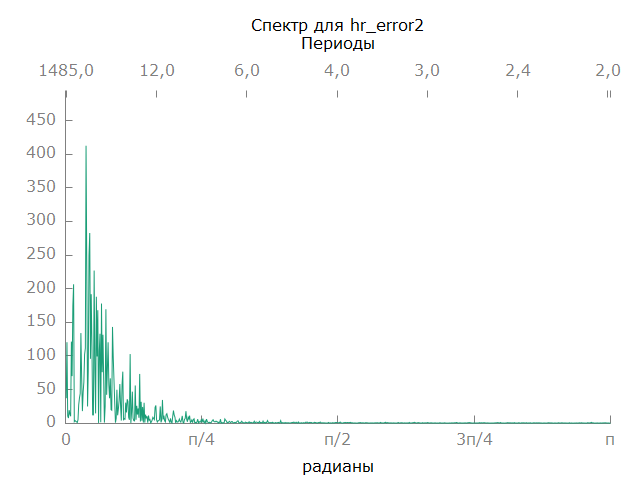
\includegraphics[width=0.5\linewidth]{../[graphics]/hr_error2_spectr.png}
	\caption{Периодограмма остаточной разности основной модели}
	\label{fig:hr_error2_spectr}
\end{figure}

При подборе порядка авторегрессии и скользящего среднего наилучший результат по критерию Акаике получился у модели ARIMA(8, 0, 7) (таблица \ref{tab:table4}). При анализе коррелограммы и периодограммы остаточной разности hr\_error3 модели ARIMA по графикам \ref{fig:hr_error3_acf_100} и \ref{fig:hr_error3_spectr} соответственно, можно сказать, что hr\_error3 визуально схожа с процессом белого шума. По критерию Бокса-Льюнга принимаем нулевую гипотезу об отсутствии автокорреляции с вероятностью ошибки первого рода 10\%.

\begin{table}[H]
\begin{center}
	
	ARIMA(8, 0, 7), использованы наблюдения 1--1485\\
	Зависимая переменная: hr\_error1\\
	Стандартные ошибки рассчитаны на основе Гессиана
	
	\vspace{1em}
	
	\begin{tabular}{lr@{,}lr@{,}lr@{,}lr@{,}l}
		&
		\multicolumn{2}{c}{Коэффициент} &
		\multicolumn{2}{c}{Ст.\ ошибка} &
		\multicolumn{2}{c}{$z$} &
		\multicolumn{2}{c}{P-значение} \\[1ex]
		const &
		$-$0&0133712 &
		0&533708 &
		$-$0&02505 &
		0&9800 \\
		$\phi_{1}$ &
		0&954470 &
		0&0531005 &
		17&97 &
		0&0000 \\
		$\phi_{2}$ &
		1&02735 &
		0&0922044 &
		11&14 &
		0&0000 \\
		$\phi_{3}$ &
		$-$0&281596 &
		0&140136 &
		$-$2&009 &
		0&0445 \\
		$\phi_{4}$ &
		$-$1&07043 &
		0&0826160 &
		$-$12&96 &
		0&0000 \\
		$\phi_{5}$ &
		$-$0&594566 &
		0&189362 &
		$-$3&140 &
		0&0017 \\
		$\phi_{6}$ &
		0&576216 &
		0&0723388 &
		7&966 &
		0&0000 \\
		$\phi_{7}$ &
		1&01328 &
		0&135282 &
		7&490 &
		0&0000 \\
		$\phi_{8}$ &
		$-$0&685049 &
		0&0776715 &
		$-$8&820 &
		0&0000 \\
		$\theta_{1}$ &
		0&368473 &
		0&0616605 &
		5&976 &
		0&0000 \\
		$\theta_{2}$ &
		$-$0&804200 &
		0&0742579 &
		$-$10&83 &
		0&0000 \\
		$\theta_{3}$ &
		$-$0&973799 &
		0&0746751 &
		$-$13&04 &
		0&0000 \\
		$\theta_{4}$ &
		$-$0&117496 &
		0&107461 &
		$-$1&093 &
		0&2742 \\
		$\theta_{5}$ &
		0&787371 &
		0&0911584 &
		8&637 &
		0&0000 \\
		$\theta_{6}$ &
		0&666557 &
		0&0674118 &
		9&888 &
		0&0000 \\
		$\theta_{7}$ &
		$-$0&336733 &
		0&0738103 &
		$-$4&562 &
		0&0000 \\
		ele\_error1 &
		0&445471 &
		0&0820600 &
		5&429 &
		0&0000 \\
		cad\_trend1 &
		$-$0&0422177 &
		0&451399 &
		$-$0&09353 &
		0&9255 \\
	\end{tabular}
	
	\vspace{1ex}
	\begin{tabular}{lrlr}
		Среднее зав. перемен & $-$3,83\textrm{e--17} & Ст. откл. зав. перемен &  8,808905 \\
		Среднее инноваций &  0,005414 & Ст. откл. инноваций &  2,102646 \\
		$R^2$ &  0,942993 & Исправленный $R^2$ &  0,942372 \\
		Лог. правдоподобие & $-$3214,469 & Крит. Акаике &  6466,939 \\
		Крит. Шварца &  6567,699 & Hannan--Quinn &  6504,494 \\
	\end{tabular}
	
	
	\vspace{1em}
	
	\begin{tabular}{llrrrrr}
		& & & Действительная часть & Мнимая часть & Модуль & Частота \\ \hline
		AR \\ 
		& Корень & 1 & $1,0304$ & $0,2333$ & $1,0565$ & $0,0354$ \\ 
		& Корень & 2 & $1,0304$ & $-0,2333$ & $1,0565$ & $-0,0354$ \\ 
		& Корень & 3 & $-0,9350$ & $0,3739$ & $1,0070$ & $0,4394$ \\ 
		& Корень & 4 & $-0,9350$ & $-0,3739$ & $1,0070$ & $-0,4394$ \\ 
		& Корень & 5 & $1,0390$ & $-0,3774$ & $1,1055$ & $-0,0555$ \\ 
		& Корень & 6 & $1,0390$ & $0,3774$ & $1,1055$ & $0,0555$ \\ 
		& Корень & 7 & $-0,3949$ & $-0,9485$ & $1,0274$ & $-0,3128$ \\ 
		& Корень & 8 & $-0,3949$ & $0,9485$ & $1,0274$ & $0,3128$ \\ 
		MA \\ 
		& Корень & 1 & $-0,9293$ & $0,3693$ & $1,0000$ & $0,4398$ \\ 
		& Корень & 2 & $-0,9293$ & $-0,3693$ & $1,0000$ & $-0,4398$ \\ 
		& Корень & 3 & $0,9882$ & $-0,3146$ & $1,0370$ & $-0,0491$ \\ 
		& Корень & 4 & $0,9882$ & $0,3146$ & $1,0370$ & $0,0491$ \\ 
		& Корень & 5 & $-0,3827$ & $-0,9511$ & $1,0252$ & $-0,3109$ \\ 
		& Корень & 6 & $-0,3827$ & $0,9511$ & $1,0252$ & $0,3109$ \\ 
		& Корень & 7 & $2,6271$ & $0,0000$ & $2,6271$ & $0,0000$ \\ \hline
	\end{tabular}
	
\end{center}
\caption{Модель статистической взаимосвязи между зависимой и независимыми переменными с учетом автокорреляции случайной составляющей.}
\label{tab:table4}
\end{table}

\begin{figure}[H]
	\centering
	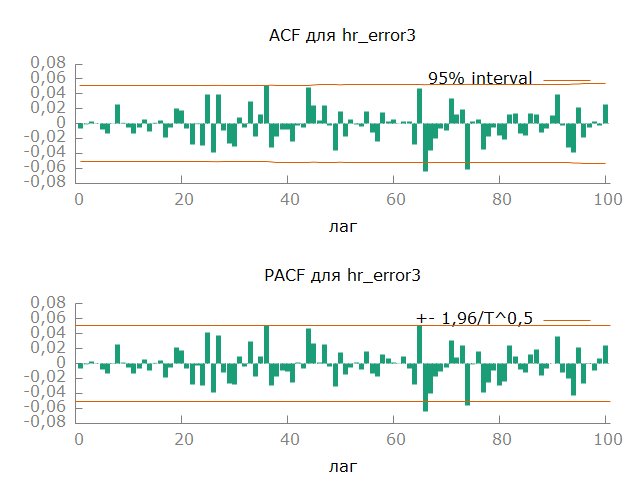
\includegraphics[width=0.5\linewidth]{../[graphics]/hr_error3_acf_100.png}
	\caption{Графики ACF и PACF остаточной разности модели ARMA}
	\label{fig:hr_error3_acf_100}
\end{figure}

\begin{figure}[H]
	\centering
	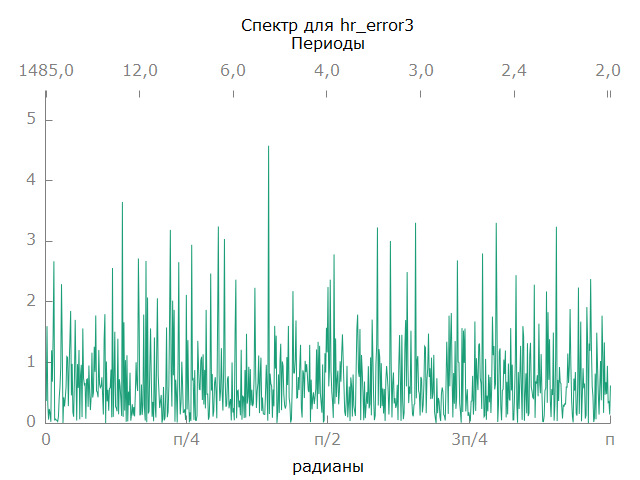
\includegraphics[width=0.5\linewidth]{../[graphics]/hr_error3_spectr.png}
	\caption{Периодограмма остаточной разности модели ARMA}
	\label{fig:hr_error3_spectr}
\end{figure}


\section{Выводы и рекомендации}
Таким образом, можно сказать, что долгосрочный тренд выявлен только в зависимой переменной Пульс. Циклические тренды выявлены во всех представленных переменных. Наиболее ярковыраженная гармоническая составляющая имеет период в 6 минут - это объясняется тем, что в среднем на прохождение круга у спортсмена уходило 6 минут. Выдающихся сезонных трендов ни в одной из представленных переменных не выявлено.  

По результатам проверки гипотез можно сделать вывод, что гипотеза 1 о том, что увеличение высоты траектории статистически связано с увеличением частоты пульса спортсмена верна. Действительно, при наборе высоты спортсмену приходится прилагать больше усилий, что отражается на частоте пульса

Однако гипотеза 2 о статистической связи каденса и пульса не подтвердилась. Это может быть связано с неточностью измерений частоты шагов спортсмена - такая технология для лыжного спорта не до конца отработана и чаще применяется, например, при анализе бега.


\end{document} % конец документа